
%\documentclass[12pt,notitlepage,aps,pra,longbibliography,nofootinbib,tightenlines]{revtex4}
%\documentclass[12pt,notitlepage,longbibliography,nofootinbib,tightenlines]{revtex4-1}

\documentclass[12pt]{article}

%\documentclass[12pt,a4]{revtex4}
%\documentclass[12pt]{article}
%\documentclass[11pt, twocolumn]{article}

%\usepackage{epsf}
\usepackage{amsmath}
\usepackage{color}
\usepackage{natbib}
%\usepackage{cite}

\RequirePackage{amsmath}
\RequirePackage{amssymb}
\RequirePackage{amsthm}
%\RequirePackage{algorithmic}
%\RequirePackage{algorithm}
%\RequirePackage{theorem}
%\RequirePackage{eucal}
\RequirePackage{color}
\RequirePackage{url}
\RequirePackage{mdwlist}

\RequirePackage[all]{xy}
\CompileMatrices
\RequirePackage{hyperref}
\RequirePackage{graphicx}
%\RequirePackage[dvips]{geometry}

\newtheorem{theorem}{Theorem}
\newtheorem{lemma}{Lemma}


\begin{document}

%\title{Representations of Pauli Operator Hamiltonians}
\title{Representations of Subsystem Code Hamiltonians}

\author{Simon Burton}
%\affiliation{Centre for Engineered Quantum Systems, School of Physics, The University of Sydney}

\date{\today}

%\begin{abstract}
%\end{abstract}

\maketitle

\begin{abstract}
\end{abstract}


% CUT HERE

\def\Complex{\mathbb{C}}
\def\C{\mathbb{C}}
\def\R{\mathbb{R}}
\def\Z{\mathbb{Z}}
%\def\Ham{\mathcal{H}} % meh..
\def\Ham{H} 
\def\Pauli{\mathcal{P}}
\def\Spec{\mbox{Spec}}
\def\Proveit{{\it (Proof??)}}
\def\GL{\mathrm{GL}}
\def\half{\frac{1}{2}}
\def\Stab{S}

\newcommand{\ket}[1]{|{#1}\rangle}
\newcommand{\expect}[1]{\langle{#1}\rangle}
\newcommand{\bra}[1]{\langle{#1}|}
\newcommand{\ketbra}[2]{\ket{#1}\!\bra{#2}}
\newcommand{\braket}[2]{\langle{#1}|{#2}\rangle}


%%%%%%%%%%%%%%%%%%%%%%%%%%%%%%%%%%%%%%%%%%%%%%%%%%%%%%%%%%%%%%%%%%%%%%%%%%%%%%%
%
%%%%%%%%%%%%%%%%%%%%%%%%%%%%%%%%%%%%%%%%%%%%%%%%%%%%%%%%%%%%%%%%%%%%%%%%%%%%%%%
%

\section{Motivating examples}

There's at least one version of mathematical dogma that would
have us perform our linear algebra without choosing a basis.
Any basis, or preferred subspace, should only come from the
operators at hand, as eigenspaces or reducible subspaces.
But by the time we have discovered these all the fun is over.
Here we are interested in 
thinking of the Hamiltonian as a matrix of transition
amplitudes that describe a dynamical processes. 
Experimental implementations of such schemes
often do come with a basis.

%The above Hamiltonian operates on a two dimensional state space.
We start our journey considering a two-dimensional state space.
This space is blessed with two basis vectors $\ket{0}$ and $\ket{1}.$
The $Z$ and $X$ operators act on these states as:
\begin{center}
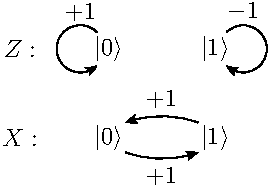
\includegraphics[]{pic-zx.pdf}
\end{center}
From this picture we can see that $Z$ acts by \emph{stabilizing} the
state $\ket{0}$ and anti-stabilizing the $\ket{1}$ state.
The $Z$ operator has been reduced 
to two operators each acting on a one dimensional subspace:
$Z = +1 \oplus -1.$
The $X$ operator serves to ``bitflip'' the state between
these two subspaces.

But what happens if we get confused and end up swapping
the $X$ and $Z$ operators? We would like to see the $X$ operator
as stabilizing / anti-stabilizing two subspaces, together with the
$Z$ operator as bitflipping between these.
The trick is to consider the \emph{orbits} of the operator
we hope to act as a stabilizer.
In this case there is only one orbit, $\ket{0}+\ket{1}$
and indeed, the $Z$ operator bitflips this to another state
$\ket{0}-\ket{1}$ that is anti-stabilized by $X.$

We are going to be considering Hamiltonians built from
summing operators of this form.
In this paper we use a ``neg-Hamiltonian'' convention,
to save complicating expressions with negative signs.
The ground space corresponds to the \emph{largest} eigenvalue.

Building a Hamiltonian from a single $X$ or $Z$ term
we can find the ground space as the stabilized space
using orbits. Then the adjacent operator acts to bitflip
between the eigenspaces.
To further elucidate this idea we turn to another example.
Now we have a hamiltonian built from three commuting and
independent operators 
$$
    \Ham = XXI + IXX + ZZZ.
$$
Starting with $\ket{000}$ we compute the orbit state
as $\ket{000}+\ket{011}+\ket{110}+\ket{101}.$
This time we have three bitflip operators
one for each of the stabilizer operators:
$ZII, IIZ, IXI.$
(We could also have chosen $IZZ, ZZI, XXX.$)
For example, $ZII$ sends the ground state to
$\ket{000}+\ket{011}-\ket{110}-\ket{101}$
which is anti-stabilized by $XXI.$
The bitflip operators form an abelian group of
order $2^3 = 8$ and by appying each element of
this group to the ground state we get a basis
of our state space, which we call a \emph{symmetry
invariant basis.}

Now we consider a four qubit example:
$$
    \Ham = XXII + IIXX + ZIZI + IZIZ.
$$
This time the terms of the Hamiltonian do not form
an abelian group.
We will call the group generated by the terms in the Hamiltonian
the \emph{gauge} group, $G$.
The stabilizers in this case will be the elements of $G$
that commute with every other element in $G.$
By inspection we see these are generated by $\Stab_0=\{XXXX, ZZZZ\}.$
and we can choose the reduced gauge generators to be $R_0=\{XXII, ZIZI\}.$
The logical operators are generated by $L_0 = \{XIXI, ZZII\},$
and then the errors $T_0$ corresponding to $\Stab_0$ will
be $\{ZZZI, IIIX\}.$
All of this can be summarized in a table of anti-commuting pairs:
\begin{center}
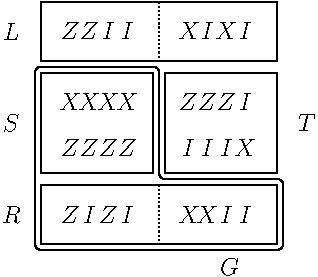
\includegraphics[]{pic-gauge4.pdf}
\end{center}
where the number of rows equals $n$ and each entry
commutes with the entries on other rows, and anticommutes
with the entry on the same row. 
If we take all the operators in the left column
we get the operators 
$\{ ZZII, XXXX, ZZZZ, ZIZI \}.$ 
These generate an abelian group 
that stabilizes the
state $\ket{\psi} = \ket{0000}+\ket{1111}.$
Let $r$ be the gauge operator $XXII$ adjacent to the 
stabilizer $ZIZI$,
The state $\ket{\psi}$ then lies in the $G-$orbit 
$$
\{\ket{\psi}, r\ket{\psi}\} = \{\ket{0000}+\ket{1111}, \ket{1100}+\ket{0011}\}.
$$
We use the $T_0$ operators $t_1=ZZZI$ and $t_2=IIIX$
to list three other $G-$orbits:
$$
\{t_1 \ket{\psi}, t_1 r\ket{\psi}\}, 
\{t_2 \ket{\psi}, t_2 r\ket{\psi}\}, 
\{t_1 t_2 \ket{\psi}, t_1 t_2 r\ket{\psi}\}.
$$
Here we have sixteen vectors forming an orthogonal basis for the state space.
They are arranged on the vertices of a cube. This cube is actually a four
dimensional hypercube, but we suppress the last dimension in
this diagram.
Such an arrangement of basis vectors has a cartesian product
structure which induces a tensor product decomposition of
the original state space.
\begin{center}
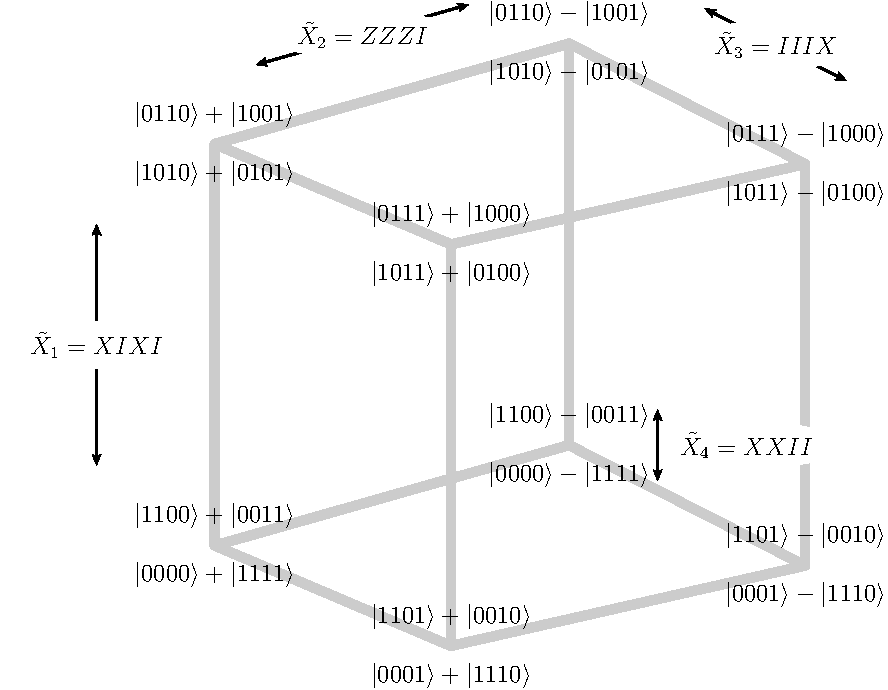
\includegraphics[width=0.9\columnwidth]{pic-operators.pdf}
\end{center}
The Hamiltonian acts on states by left multiplication.
Because this action
is a sum of gauge group elements,
it will decompose into blocks,
one for each $G-$orbit.
We depict this action as a weighted graph, where we omit edges
with zero weight:
\begin{center}
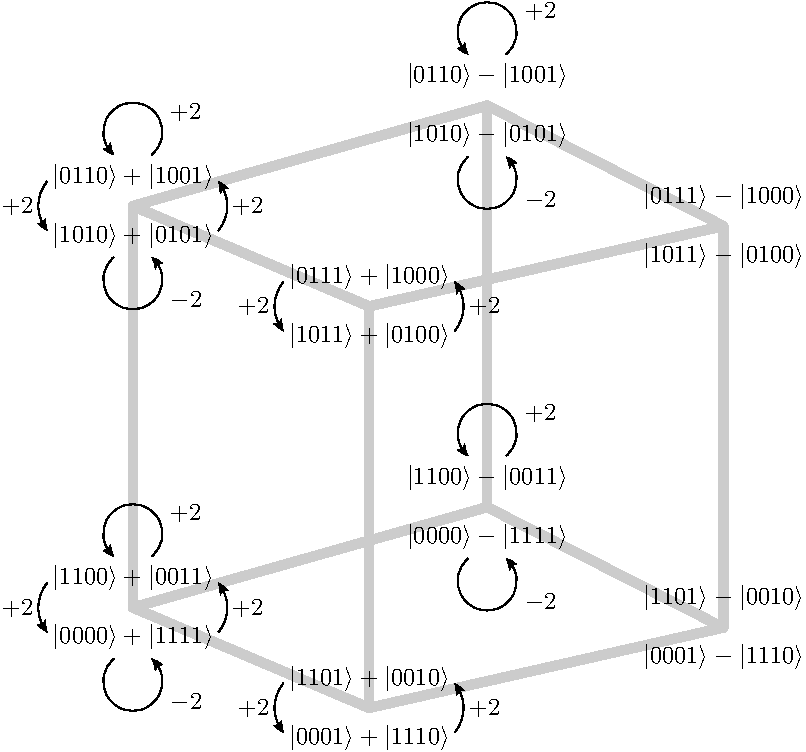
\includegraphics[width=0.9\columnwidth]{pic-orbit.pdf}
\end{center}

\def\Xt{\tilde{X}}
\def\Zt{\tilde{Z}}

\begin{align*}
\Ham &= XXII + IIXX + ZIZI + IZIZ \\
  &= \Xt_4 + \Zt_2\Xt_4 + \Zt_4 + \Zt_3\Zt_4 \\
  &= (I+\Zt_2)\Xt_4 + (I+\Zt_3) \Zt_4.
\end{align*}

Using the symmetry invariant basis computed from the orbits we
can write the matrix for the Hamiltonian in
block diagonal form:
$$
\Ham = 
\left( \begin{array}{cccc}
2(X+Z) & 0 & 0 & 0 \\
0  & 2X & 0 & 0 \\
0  & 0 & 2Z & 0 \\
0  & 0 & 0 & 0 \\
\end{array} \right) \otimes I
$$



\section{Representation theory}

\subsection{The Pauli group}

The Pauli group $\Pauli_1$ is normally 
defined as a set of matrices closed under
matrix multiplication, but we can define
it abstractly
as the group generated
by the (abstract) elements $\{\omega, X, Z\}$ with
relations as follows:
$$
\omega^2=I,\ X^2=I,\ Z^2=I,\ \omega X\omega X=I,\ \omega Z\omega Z=I,\ \mbox{and}\  \omega ZXZX=I,
$$
where $I$ is the group idenity.
Actually, $\omega $ is generated by $X$ and $Z$, so
it is not necessary to include $\omega $ in the generating set,
but here it simplifies the relations.
\footnote{We leave out $Y$ because...}
This group has eight elements, and is isomorphic to the dihedral group $D_4$,
the symmetry group of a square.

To define
the {\it $n$-qubit Pauli group} $\Pauli_n$, 
we use the $2n+1$ element 
generating set $\{\omega , X_1, .., X_n, Z_1, .., Z_n\}$
with relation $\omega^2=I$ as before, and
\begin{equation}\label{presentation}
\begin{array}{c}
X_i^2=I,\ Z_i^2=I,\ \omega X_i\omega X_i=I,\ \omega Z_i\omega Z_i=I,\ \omega Z_iX_iZ_iX_i=I, 
\mbox{\ for\ } i=1,...n,\\
Z_iX_jZ_iX_j=I, \mbox{\ for\ } i, j = 1,..,n,\ i\ne j.
\end{array}
\end{equation}

This abstract approach to the definition of a group is known as
a group {\it presentation}. In general, this is a set of
generators together with a set of relations satisfied
by these generators.

Note that each of the generators squares to the identity,
and of these, only $\omega$ commutes with every element of $\Pauli_n.$
%Note that $\omega$ commutes with all elements of $\Pauli_n$
%and squares to the idenity, 
Therefore we will write $\omega$ as $-I,$
similarly $\pm I$ will denote the
set $\{\omega, I\},$ and $-X$ is $\omega X$, etc.

We write the group commutator as
$[[g, h]]:=ghg^{-1}h^{-1}$
and note the important commutation relation:
$$
    [[Z_i, X_j]] = 
    \left\{ \begin{array}{ll}
 -I &\mbox{if}\ i=j,\\
 I &\mbox{if}\ i\ne j.\end{array}\right.
$$
If we take an arbitrary $g\in \Pauli_n$
written as a product of the generators,
it follows that we can rewrite this
product uniquely as %in an ordered fashion:
$ g = \pm g_1 ... g_n $
where each $g_i$ is one of $I, Z_i, X_i$ or $X_i Z_i$
for $i=1,..,n.$
Therefore, the size of the
Pauli group is 
$$
    |\Pauli_n| = 2^{2n+1}.
$$

%Elements of $\Pauli_n$ that consist of
%products of only $I$ or $X$ will
%be call $X$-type elements (or operators)
%and similarly $Z$-type elements are 
%products of only $I$ or $Z$.
The subgroup of $\Pauli_n$ generated by
the elements $\{X_1,...,X_n\}$ % $\{X_i\}_{i=1,..,n}$ 
is denoted $\Pauli_n^X.$ These are the $X$-type
elements. Similarly,
 $\{Z_1,...,Z_n\}$ generates % $\{Z_i\}_{i=1,..,n}$ 
the subgroup of $Z$-type elements $\Pauli_n^Z$.


\subsection{Subgroups of the Pauli group}

We now define an {\it $n-$qubit gauge group} to be 
any non-abelian subgroup $G$ of $\Pauli_n,$
defined by a set of generators $G_0\subset \Pauli_n,$
%for some subgroup $G$ of $\Pauli_n:$
$$ G := \langle G_0\rangle.$$
%We will assume $G$ is not abelian, which 
%%is equivalent to the condition that $-I\in G.$ % No! {-I, I} is abelian...
%implies that $-I\in G.$
Because $G$ is not abelian, it follows that $-I\in G.$
We also restrict $G_0$ to only contain Hermitian operators,
which is equivalent to requiring that $g^2=I$ for all $g\in G_0.$

Now let $\Stab$ be the largest subgroup of $G$ not containing
$-I.$
$\Stab$ is then an abelian subgroup,
also known as the {\it stabilizer} subgroup.
%(Note that each of the stabilizers commutes with the Hamiltonian.)
$G$ decomposes as a direct product:
$$G = \Stab\times R,$$
where $R\cong P_r$ for some $1\le r\le n,$
and $\Stab\cong \Z_2^{m}$ for $0\le m<n.$
Therefore, 
$$|G| = |\Stab| |R| = 2^{m+2r+1}.$$
We call $R$ the {\it reduced gauge group}.
We consider both $\Stab$ and $R$ to be subgroups of $G.$
%Let $\phi:P_r\to R$ be a group isomorphism,
Let $\phi:R\to P_r$ be a group isomorphism,
%then $R_0 := \{\phi(X_i), \phi(Z_i)\}_{1\le i\le r}$
%then $R_0 := \{\phi(X_i), \phi(Z_i)\}_{i=1,..,r}$
then $R_0 := \{\phi^{-1}(X_i), \phi^{-1}(Z_i)\}_{i=1,..,r}$
is a set of independent generators of $R.$
We also let $\Stab_0$ be a set of $m$ independent generators of $\Stab.$

To find the cosets of $G$ in $\Pauli_n$ we take
the group closure of $G-\Pauli_n$; when this is non-empty
we only need to add $I$ and $-I.$
This is another
gauge group, whose reduced gauge group is known as
the {\it logical} operators $L$, and whose 
stabilizer subgroup is known as the {\it error} operators $T.$
Now any coset of $G$ can be written as $ltG$ with
$l\in L$ and $t\in T.$
The size of $T$ equals the size of $\Stab$: $|T|=|\Stab|=2^m.$
If we let $L_0$ be an independent generating set for $L$
then we have the important formula:
\begin{align}
n &= \frac{1}{2}|L_0| + |\Stab_0| + \frac{1}{2}|R_0|\\
  &= k + m + r
\end{align}
We summarize the information in this section in a table
of Pauli group elements arranged in
two columns and $n$ rows:
\begin{center}
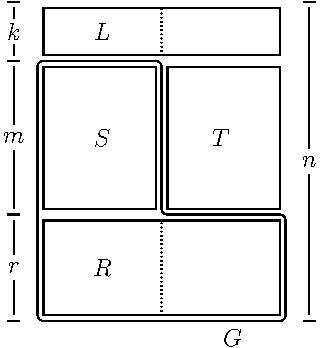
\includegraphics[]{pic-canonical.pdf}
\end{center}
Here we show the $2n$ generators of $\Pauli_n$ arranged 
so that each row contains a pair of generators,
where each such generator anti-commutes with the operator on the same row and
commutes with all the other operators in the table.
Note that this is exactly the definition of the Pauli group
via a presentation given in the previous section.
Furthermore, the table shows $2k$ generators
of $L$, $m$ generators each for $S$ and $T,$ and $2r$
generators of $R.$
The gauge group $G$ encloses $R$ and $S$, and one can
immediately see how $L$ and $T$ also form a gauge group.


\subsection{Representations of the Pauli group}

We now define the
{\it Pauli representation} 
of the Pauli group as a group homomorphism:
$$
    \rho_{\mathrm{pauli}} : \Pauli_n \to \GL(\Complex[2^n])
$$
where $\Complex[2^n]$ is the $2^n$-dimensional state space of $n$ qubits.
On the independent generators 
$\{X_1, .., X_n, Z_1, .., Z_n\},\ \rho_{\mathrm{pauli}}$
is defined as the following tensor product of $2\times 2$ matrices:

%$$
%\rho_{\mathrm{pauli}}(X_i) := \bigotimes_{j=1}^n \left\{ \begin{array}{ll}
%\left( \begin{array}{ll}
%1&0\\
%0&1\end{array} \right) &\mbox{for $j\ne i$,}\\
%\\
%\left( \begin{array}{ll}
%0&1\\
%1&0\end{array} \right) &\mbox{for $j=i$} \end{array}
%\right\},\ 
%\rho_{\mathrm{pauli}}(Z_i) := \bigotimes_{j=1}^n \left\{ \begin{array}{ll}
%\left( \begin{array}{ll}
%1&0\\
%0&1\end{array} \right) &\mbox{for $j\ne i$,}\\
%\\
%\left( \begin{array}{rr}
%1&0\\
%0&-1\end{array} \right) &\mbox{for $j=i$}\end{array}
%\right\}.
%$$

\begin{align*}
\rho_{\mathrm{pauli}}(X_i) := &\bigotimes_{j=1}^n \left\{ \begin{array}{ll}
\left( \begin{array}{ll}
0&1\\
1&0\end{array} \right) &\mbox{for $j=i$}\\
\\
\left( \begin{array}{ll}
1&0\\
0&1\end{array} \right) &\mbox{for $j\ne i$} \end{array}
\right.\\
\rho_{\mathrm{pauli}}(Z_i) := &\bigotimes_{j=1}^n \left\{ \begin{array}{ll}
\left( \begin{array}{ll}
1&0\\
0&-1\end{array} \right) &\mbox{for $j=i$}\\
\\
\left( \begin{array}{rr}
1&0\\
0&1\end{array} \right) &\mbox{for $j\ne i$}\end{array}
\right.
\end{align*}

%on $n$ qubits, $\Pauli_n,$
%as the set of $n$-fold tensor products
%of the matrices $\pm I, X, Z:$
%$$
%I = \left( \begin{array}{ll}
%1&0\\
%0&1\end{array} \right),\quad
%X = \left( \begin{array}{ll}
%0&1\\
%1&0\end{array} \right),\quad
%Z = \left( \begin{array}{ll}
%1&0\\
%0&-1\end{array} \right).
%$$

Normally the image of 
$\rho_{\mathrm{pauli}}$ is thought of as the
Pauli group itself, and we are indeed free to think
that way because $\rho_{\mathrm{pauli}}$ is a group
isomorphism.

Given a group representation $\rho:G\to GL(V)$
the {\it character} of $\rho$ is a function
$\chi_\rho:G\to \Complex$ given by
$$
    \chi_\rho(g) = \mbox{Tr}\ \rho(g).
$$

Given two functions $u,v : G \to \Complex$ 
we define the following inner product:
$$
    \langle u, v \rangle := \frac{1}{|G|} \sum_{g\in G} u(g) \overline{v(g)}.
$$

The character of the Pauli representation, $\chi_{{pauli}}:\Pauli_n\to\Complex$
is given by:
$$
\chi_{{pauli}}(g) = \sum_{v \in basis} \langle v | \rho_{{pauli}}(g) | v \rangle
    = \left\{ \begin{array}{ll}
 \pm 2^n &\mbox{if}\ g=\pm I\\
 0 &\mbox{otherwise}\end{array}\right.
$$

Since $|P_n|=2^{2n+1}$ it follows that
$\langle\chi_{pauli},\chi_{pauli}\rangle = 1$ and
so $\rho_{pauli}$ is an irreducible representation of $\Pauli_n.$

%It turns out %(see Appendix for details)
%that $\rho_{\mathrm{pauli}}$ is an
%irreducible representation ({\it irrep}) of $\Pauli_n$. 
The only other irreps of $\Pauli_n$ are 
the $1$-dimensional irreps $\rho:\Pauli_n\to\Complex$
defined on the independent generators as:
    $$ \rho(X_i) = \pm 1,\quad \rho(Z_i) = \pm 1.$$

So we have $2^{2n}$ many $1$-dimensional irreps,
and a single $2^n$-dimensional irrep.
Summing the squares of the dimensions
shows that we have a complete set of irreps of $\Pauli_n.$

\subsection{Representations of stabilizer groups}

Any abelian subgroup $\Stab\subset \Pauli_n$
that does not contain $-I$ we call a stabilizer group.
The reason for this name is...



\subsection{Representations of gauge groups}

%Our next job will be to find the irreps of {\it subgroups} of $\Pauli_n.$
Although $\rho_{\mathrm{pauli}}$
restricted to a gauge group $G\subset\Pauli_n$ serves as a representation
of $G$ it is no longer irreducible.
Our aim will be to decompose $\rho_{\mathrm{pauli}}$ into irreps of $G.$

The $1$-dimensional irreps $\rho:G\to \Complex,$
are now defined by
specifying the action of $\rho$ on the independent generators:
$$
    \rho(h)=\pm 1\ \mbox{for}\ h\in \Stab_0,
    \quad \rho(\phi^{-1}(X_i)) = \pm 1,\quad \rho(\phi^{-1}(Z_i)) = \pm 1.
$$
This gives all $2^{m+2r}$ of the $1$-dimensional irreps.
%These will turn out not to be used below.

The $2^r$-dimensional irreps are given by:
$$
    \rho(h) = \pm I^{\otimes r}\ \mbox{for}\ h\in \Stab_0,
    \quad \rho(\phi^{-1}(X_i)) = X_i,\quad \rho(\phi^{-1}(Z_i)) = Z_i.
$$
We are free to choose the signs of the $\rho(h)$ for each $h\in \Stab_0.$
Hence there are $2^m$ many of these irreps.
Each such choice corresponds to the choice of a {\it syndrome} vector $s(h)=\pm 1$, for $h \in \Stab_0,$
or alternatively, choice of an element $t\in T:$
$$
    \rho^1_t(h) = \left\{ \begin{array}{ll}
 I^{\otimes r}\ &\mbox{if $th=ht$}\\
 -I^{\otimes r}\ &\mbox{if $th=-ht$}\end{array} \right. %\right\}\mbox{for}\ h\in \Stab_0.
$$

%Finally, there are $2^m$ many $2^r$-dimensional irreps $\rho_t$
%which are labelled by $t\in T$ and defined as
%$$
%    %\rho_t(h)=\pm I^{\otimes 2^r}\ \mbox{for}\ h\in \Stab_0,
%    %\rho_t(h)= [t,h] = th^{-1}th^{-1} = \pm I^{\otimes 2^r}\ \mbox{for}\ h\in \Stab_0,
%    \rho_t(h) = \left\{ \begin{array}{ll}
% I^{\otimes 2^r}\ &\mbox{if $th=ht$}\\
% -I^{\otimes 2^r}\ &\mbox{if $th=-ht$}\end{array} \right\}\mbox{for}\ h\in \Stab_0,
%    \quad \rho_t(\phi^{-1}(X_i)) = X_i,\quad \rho_t(\phi^{-1}(Z_i)) = Z_i.
%$$

%For $G$ a subgroup of $\Pauli_n$, and decomposition
Because $G$ decomposes 
into a direct product $G=\Stab\times \Pauli_r$ we have the
following representations:
$$
    \rho_t(g) = \rho^1_t(h) \rho^r_{pauli}(g'),
$$
where $g=hg'$, $h\in \Stab$, $g'\in \Pauli_r$ 
%and $\rho_1(h)$ is a $1$-dimensional representation of $\Stab$.
and $\rho^r_{pauli}$ is the $r$-qubit Pauli representation.
The character for this representation is:
$$
\chi_{t}(hg') = \rho_t^1(h) \sum_{v \in basis} \langle v | \rho^r_{{pauli}}(g') | v \rangle
    = \left\{ \begin{array}{ll}
 \pm 2^r\rho_t^1(h) &\mbox{if}\ g'=\pm I\\
 0 &\mbox{otherwise}\end{array}\right.
$$

We have that $|G|=2^{2r+m+1}$ and so
$\langle\chi_{t},\chi_{t}\rangle = 1$ and
$\rho_t$ is an irreducible representation of $G.$
We now count the occurances of 
this representation in $\rho^r_{pauli}$:
\begin{align*}
\langle\chi^r_{pauli},\chi_{t}\rangle &= \frac{1}{|G|}\sum_{g\in G} \chi^r_{pauli}(g)\overline{\chi_{t}(g)} \\
&= \frac{1}{2^{2r+m+1}} \sum_{g=\pm I} 2^n 2^r = \frac{2^{n+1+r}}{2^{2r+m+1}} = 2^k
\end{align*}
where $k$ is the number of logical qubits so that $n=r+m+k.$

%\noindent{\bf Theorem.}
%Using characters one can show that
%on a subgroup $G$ of $\Pauli_n$ the
In summary, the Pauli representation decomposes into 
$2^m$ many irreps $\rho_t,$ 
each with dimension $2^r,$ 
and appearing with multiplicity $2^k:$
$$
    \rho_{\mathrm{pauli}} = \bigoplus_{l\in L, t\in T} \rho_t.
$$
%where we label the $2^r$-dimensional irreps by $t\in T.$
%See appendix for details.

\subsection{Symmetry invariant basis}

In general, given a representation $\rho:G\to \GL(V)$
and the character of some irreducible representation $\chi:G\to \C$
the following operator 
$P:V\to V$
projects onto the subspace on which
this irreducible representation acts:
$$
    P := \frac{d}{|G|} \sum_{g\in G} {\overline{\chi(g)}} \rho(g).
$$
where $d$ is the dimension of the irreducible representation.
We can use this to calculate projectors onto the irreps $\rho_t$ in $\rho_{pauli}$:
\begin{align*}
P_t &= \frac{d}{|G|} \sum_{g\in G} \overline{\chi_t(g)} \rho_{pauli}(g) \\
    &= \frac{d}{|G|} \sum_{h\in \Stab}\sum_{g\in R} \overline{\chi_t(hg)} \rho_{pauli}(hg) \\
    &= \frac{d}{|G|} 2^{2r} \sum_{h\in \Stab} {\rho^1_t(h)} \rho_{pauli}(h) \\
    &= \frac{1}{2^m} \sum_{h\in \Stab} {\rho^1_t(h)} \rho_{pauli}(h).
\end{align*}

We can also write this as a product of projectors onto
the $\pm 1$ eigenspaces of stabilizers $\rho_{pauli}(h)$ for $h\in \Stab.$
Choose generators $h_1,...,h_m$ of $S$
and then the projectors onto the $\pm 1$ eigenspace of $\rho_{pauli}(h_i)$ are
$$
P^i_t = \frac{1}{2} \bigl(I^{\otimes n} \pm \rho_{pauli}(h_i) \bigr)
$$
and we see that 
$$
P_t = \prod_{i=1,...,m} P^i_t 
    = \frac{1}{2^m} \bigl(I^{\otimes n} \pm \rho_{pauli}(h_1)\bigr)
    ...\bigl(I^{\otimes n} \pm \rho_{pauli}(h_m)\bigr).
$$
This projector will have rank $2^{k+r}$ and
$$
U := \sum_{t\in T} P_t
$$
is a unitary transformation that sends
physical qubits to encoded qubits.


\section{The Hamiltonian}

The Hamiltonian of interest is 
an operator $\Ham:\Complex[2^n]\to\Complex[2^n]$:
%and normally defined
%as the negative sum of terms from $G_0,$ but here
%we will reverse the sign:
$$ \Ham := \sum_{g\in G_0} \rho_{\mathrm{pauli}}(g).$$
Using the above decomposition we find:
\begin{align*}
    \Ham &= \sum_{g\in G_0}\ \bigoplus_{l\in L, t\in T}\ \rho_t(g)\\
         &= \bigoplus_{l\in L, t\in T} \sum_{g\in G_0}\ \rho_t(g).
\end{align*}
%The goal is to decompose $\Ham$ into blocks as
%$$
%    \Ham = \bigoplus_{\mathrm{irrep}\rho} \sum_{g\in G_0}\ \rho(g),
%$$
We will notate each block as
$\Ham_t := \sum_{g\in G_0}\rho_t(g)$
for each irrep $\rho_t$ appearing in $\Ham.$

More generally, we can assign (real valued) weights
to each operator in $G_0,$ that is
$w:G_0\to\R,$
and 
\begin{align*}
    \Ham = \sum_{g\in G_0} w(g) \rho_{\mathrm{pauli}}(g)
            = \bigoplus_{l\in L, t\in T} \sum_{g\in G_0}\ w(g) \rho_t(g).
\end{align*}

%%%%%%%%%%%%%%%%%%%%%%%%%%%%%%%%%%%%%%%%%%%%%%%%%%%%%%%%%%%%%%%%%%%%%%%%%%%%%%%
%
%%%%%%%%%%%%%%%%%%%%%%%%%%%%%%%%%%%%%%%%%%%%%%%%%%%%%%%%%%%%%%%%%%%%%%%%%%%%%%%
%

\section{Applications}

In the following applications we will make the identification
between $g$ and $\rho_{pauli}(g)$.
So terms such as $Z$ and $X$ are understood
to be the corresponding Pauli linear operators.

%%%%%%%%%%%%%%%%%%%%%%%%%%%%%%%%%%%%%%%%%%%%%%%%%%%%%%%%%%%%%%%%%%%%%%%%%%%%%%%
%
%%%%%%%%%%%%%%%%%%%%%%%%%%%%%%%%%%%%%%%%%%%%%%%%%%%%%%%%%%%%%%%%%%%%%%%%%%%%%%%
%

\subsection{2D compass model}

Here we consider the two-dimensional compass model \cite{Bacon2006}.
We coordinatize the qubits on a square 
lattice of\ $l\times l$\ sites,
$(i, j)$\ for\ $1\le i, j\le l.$
This gives $n = l^2.$
For the single qubit Pauli operators acting on site
$(i, j)$ we coordinatize with subscripts $ij$, 
with $i$ and $j$ understood modulo $l$.
The generators of the gauge group are
$$
    G_0 = \big\{ X_{ij}X_{i,j+1},\ Z_{ij}Z_{i+1,j}\ \mbox{for}\ 1\le i, j\le l\big\}.
$$
We write generators of the reduced
gauge group in anti-commuting pairs:
$$
    R_0 = \big\{ X_{i1}X_{ij},\ Z_{1j}Z_{ij}\ \mbox{for}\ 2\le i, j\le l\big\}.
$$
This makes it clear the isomorphism $\phi : R \to \Pauli_r$ to use,
and we again use pairs $i,j$ to coordinatize $\Pauli_r$:
$$
    \phi(X_{i1}X_{ij}) = X_{i-1,j-1}, \ \ \phi(Z_{1j}Z_{ij}) = Z_{i-1,j-1},\ \mbox{for}\ 2\le i, j\le l.
$$
The generators for the stabilizers are
$$
    \Stab_0 = \big\{ \prod_{i=1}^l X_{ij}X_{i,j+1},\ \prod_{i=1}^l Z_{ji}Z_{j+1,i}\ \mbox{for}\ 1\le j\le l-1\big\}.
$$
The logical operators are generated by $L_0 = \big\{ \prod_i X_{i1}, \prod_j Z_{1j} \}.$
These sets have cardinalities:
$$|G_0|=2l^2,\ |R_0| = 2(l-1)^2,\ |\Stab_0| = 2(l-1).$$
%And we note that $\frac{1}{2}|L_0| + |\Stab_0| + \frac{1}{2}|R_0| = n.$
And we note that $k+m+r=n$ is satisfied.
%Now we can define the irreps of $G$.
Now we write down the values of the
irreps on the gauge operators.
Here we define each irrep using a pair 
of syndrome vectors $s_X$ and $s_Z:$
\begin{align*}
\rho(X_{i1} X_{i2}) &= X_{i-1,1} &
%\rho(Z_{1i} Z_{2i}) &= Z_{1,i-1} &\mbox{for}\ 2\le i\le l\\
\rho(Z_{1i} Z_{2i}) &= Z_{1,i-1} \\&&&\mbox{for}\ 2\le i\le l\\
\rho(X_{il} X_{i1}) &= X_{i-1,l-1} &
%\rho(Z_{li} Z_{1i}) &= Z_{l-1,i-1} &\mbox{for}\ 2\le i\le l\\
\rho(Z_{li} Z_{1i}) &= Z_{l-1,i-1} \\&&&\mbox{for}\ 2\le i\le l\\
\rho(X_{ij} X_{i,j+1}) &= X_{i-1,j-1} X_{i-1,j} &
%\rho(Z_{ji} Z_{j,i+1}) &= Z_{j-1,i-1}Z_{j,i-1} &\mbox{for}\ 2\le i\le l, 2\le j<l\\
\rho(Z_{ji} Z_{j,i+1}) &= Z_{j-1,i-1}Z_{j,i-1} \\&&&\mbox{for}\ 2\le i\le l, 2\le j<l\\
\rho(X_{1j} X_{1,j+1}) &= s_X(j-1) \prod_{i=1}^{l-1} X_{i,j-1} X_{ij} &
%\rho(Z_{j1} Z_{j+1,1}) &= s_Z(j-1) \prod_{i=1}^{l-1} Z_{j-1,i} Z_{ji} &\mbox{for}\ 2\le j<l\\
\rho(Z_{j1} Z_{j+1,1}) &= s_Z(j-1) \prod_{i=1}^{l-1} Z_{j-1,i} Z_{ji} \\&&&\mbox{for}\ 2\le j<l\\
\rho(X_{11} X_{12}) &= \prod_{j=1}^{l-1}s_X(j) \prod_{i=1}^{l-1} X_{i1} &
\rho(Z_{11} Z_{21}) &= \prod_{j=1}^{l-1}s_Z(j) \prod_{i=1}^{l-1} Z_{1i}.
\end{align*}
Note the transposition symmetry between the $X$ and $Z$-type operators.
We sum all these terms to find 
the form of the hamiltonian in each block:
$$
\Ham_\rho = \sum_{g\in G_0} \rho(g) = \sum_{1\le i,j<l} \rho(X_{ij}X_{i,j+1}) + \rho(Z_{ij}Z_{i+1,j}).
$$
We note that in \cite{Brzezicki2013}, they perform a
spin transformation of the compass model
which also results in a $(l-1)\times(l-1)$ lattice
of spins and identical Hamiltonian except for some signs.

%%%%%%%%%%%%%%%%%%%%%%%%%%%%%%%%%%%%%%%%%%%%%%%%%%%%%%%%%%%%%%%%%%%%%%%%%%%%%%%
%
%%%%%%%%%%%%%%%%%%%%%%%%%%%%%%%%%%%%%%%%%%%%%%%%%%%%%%%%%%%%%%%%%%%%%%%%%%%%%%%
%

\subsection{Kitaev honeycomb model}


\begin{figure*}[th!]
\begin{center}
        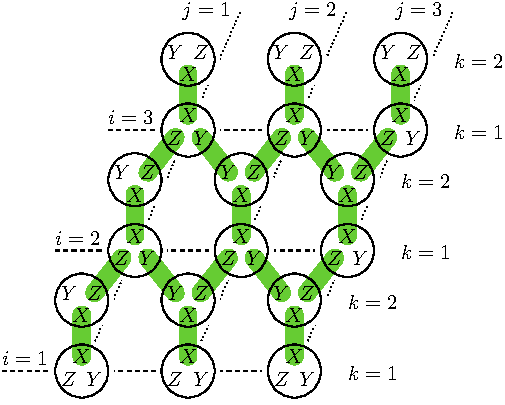
\includegraphics[width=0.6\columnwidth]{fig_00.pdf}
\caption{
Gauge generators have support on the edges of the honeycomb lattice.
Qubits here are depicted as circles.
}
\label{honeycomb}
\end{center}
\end{figure*}


The Kitaev honeycomb model \cite{Kitaev2006} is built from spins on
the sites of a hexagonal lattice. 
The lattice of linear size $l$ has $n=2l^2$ sites
which we coordinatize using integer triples $i, j, k$
with $1\le j, k\le l$ and $k=1, 2.$
We use periodic boundary conditions so $i, j$ are
to be taken modulo $l$.
See figure \ref{honeycomb}.
The edges of the lattice are in one-to-one
correspondence with the generators $G_0$:
$$
G_0 := \big\{X_{ij1}X_{ij2},\ Z_{ij2}Z_{i+1,j1},\ Y_{ij1}Y_{i-1,j+1,2}
\ \mbox{for}\ 1\le i,j\le l\big\}.
$$
Note that we make the definition $Y:=XZ$ for each site.

Stabilizers are generated from closed strings of
gauge operators. 
For example, each hexagon gives a stabilizer
\begin{align*}
h_{ij}:&= 
X_{ij1}X_{ij2}
Z_{ij2}Z_{i+1,j1}
Y_{i+1,j1}Y_{i,j+1,2}
X_{i,j+1,2}X_{i,j+1,1}
Z_{i,j+1,1}Z_{i-1,j+1,2}
Y_{i-1,j+1,2}Y_{ij1}
\\
&= 
Z_{ij1} Y_{ij2} X_{i+1,j1}
Z_{i,j+1,2} Y_{i,j+1,1} X_{i-1,j+1,2}.
\end{align*}

And the two homologically non-trivial loops
give stabilizers:
$$
h_v := \prod_{i=1}^l Y_{i11} Y_{i12},\ \ 
h_h := \prod_{j=1}^l X_{1j2} X_{2j1}.
$$

This gives independent stabilizer generators $\Stab_0$
from each hexagon, less one, as well as $h_v$ and $h_h.$
%two homologically non-trivial loops.
The number of hexagons is $\frac{1}{2}n$ and
so we find $|\Stab_0|=\half n+1.$
There are no logical operators, so we
must have $|R_0|=n-2.$

\begin{figure*}[th!]
\begin{center}
        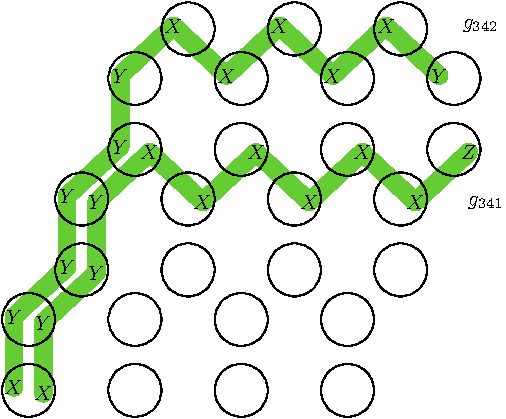
\includegraphics[width=0.5\columnwidth]{fig_01.pdf}
%\caption{Two elements $g_{341}$ and $g_{342}$ of the set $R_0$}
\caption{Two elements of the set $R_0$ corresponding
to $i=3$, $j=4$ and $k=1,2.$}
\label{jaws}
\end{center}
\end{figure*}

Now we construct a set of string operators $R_0$,
one for each site on the lattice, except for
the two sites $(1,1,1)$ and $(1,1,2).$
Each string $g_{ijk}\in R_0$
is constructed as the product of
gauge operators along a path starting at
$(1,1,1)$ and terminating at $(i,j,k).$
See figure \ref{jaws}.
Each such path is built from two ``straight''
path segments, first in the $i$ direction
and then in the $j$ direction. 
The paths for operators $g_{ij1}$ and
$g_{ij2}$ coincide along the $i$ direction
but become disjoint in the $j$ direction:
the $g_{ij1}$ path goes around the bottom
of the hexagons and the $g_{ij2}$ path
goes around the top.
%In \cite{Kells2009} they introduce a set of
%mutually anti-commuting string operators $R_0.$
With periodic boundary conditions $R_0$ forms an
independent generating set of $R$ of size $n-2.$

We construct an isomorphism $\phi: R\to \Pauli_r$
by sending elements of $R_0$ bijectively
to the following independent generating
set of $\Pauli_r$:
$$
\big\{c_{2j}:=Z_1...Z_{j-1} X_j,\ c_{2j+1}:=Z_1...Z_{j-1} Y_j\ \ \mbox{for}\ 1\le j\le r\big\}.
$$
The bijection is constrained 
by setting $\phi(g_{ij1}):=c_{2j'+1}$
and $\phi(g_{ij2}):=c_{2j'}$
where $j'$ is chosen uniquely for each $i, j.$
The $c_j$ are paired Majorana fermion operators \cite{Kitaev2006}.

%We construct an isomorphism $\phi: R\to \Pauli_r$
%by setting $\phi(g_{ij1}):=c_{2j'}$
%and $\phi(g_{ij2}):=c_{2j'+1}$
%%we map 
%%elements of $R_0$ to the following independent generating
%where the $c_j$ form the following independent generating
%set of $\Pauli_r$:
%$$
%%\big\{\prod_{i=1}^{j-1} Z_i X_j,\ \prod_{i=1}^{j-1} Z_i Y_j\ \mbox{for}\ 1\le j\le r\big\}.
%\big\{c_{2j}:=Z_1...Z_{j-1} X_j,\ c_{2j+1}:=Z_1...Z_{j-1} Y_j\ \ \mbox{for}\ 1\le j\le r\big\}.
%$$

We check this is a group homomorphism by showing that relations
satisfied by elements of $R_0$ are satisfied by
their images under $\phi.$
All such relations are either of the form
$g^2=~\pm~I$, $gg'=\pm~g'g$, or
products thereof.
So it is sufficient to check squares of
elements and commutation relations.
Every element of $R_0$ anticommutes with
every other element of $R_0$, and this is true also
of the $c_j.$
Also, $g_{ij1}^2=-I$ and $g_{ij2}^2=I$ 
is preserved by $\phi$ because $c_{2j}^2=I$ and $c_{2j+1}^2=-I$.
Finally, $\phi$ is an isomorphism
because it is a bijection of two independent
generating sets.

The next step is to write each element of $G_0$
as a product of reduced gauge operators and stabilizers.
The key thing to note is that the product of two
operators $g_{ijk}, g_{i'j'k'}\in R_0$ gives a string
operator between the sites $(i,j,k)$ and $(i',j',k')$.
And {\it any} string operator between these
two sites can then be generated by using stabilizers to
``deform'' the string $g_{ijk}g_{i'j'k'}.$
For example, taking the product
of two operators from $R_0$ that differ
by one path segment gives the following:
\begin{align*}
Z_{ij2}Z_{i+1,j,1} &= g_{ij2} g_{i+1,j,1} \\
%&\mbox{for}\ \  1\le i<l,\ 1\le j\le l, \ \ \mbox{except}\ \  (i,j)=(1,1) \ \ \mbox{or}\ \ (l,1)\\
Y_{i+1,j,1}Y_{i,j+1,2} &= g_{i+1,j,1}g_{i,j+1,2}
%&\mbox{for}\ \  1\le i,j\le l, \ \ \mbox{except}\ \  (i,j)=(1,1) \ \ \mbox{or}\ \ (l,1).
\end{align*}
We need the homologically non-trivial stabilizers to get these:
\begin{align*}
Z_{lj2}Z_{1j1} &= h_v g_{lj2} g_{1j1} &\mbox{for}\ \  2\le j\le l
\end{align*}
And the $X_{ij1}X_{ij2}$
gauge operators can be generated
by the product of 
$g_{ij1}g_{ij2}$ and the enclosed hexagon stabilizers:
$$X_{ij1}X_{ij2}=g_{ij1}g_{ij2}\prod_{j'=1}^{j-1} h_{ij'}.$$

The only $G_0$ operators that are not 
quadratic in $R_0$ operators are the five
operators that touch either of the sites
$(1,1,1)$ or $(1,1,2)$.

So each block in the Hamiltonian
is seen to be quadratic in the $c_j$ plus
five other Pauli operator terms which we denote as $\Lambda_\rho$:
$$
    \Ham_\rho = \sum_{ij} \Gamma_{ij}(\rho) c_i c_j + \Lambda_\rho
$$
The coefficients $\Gamma_{ij}$ are dependant on the irrep $\rho.$

%A similar analysis applies to the ising model, Jordan-Wigner... 
%http://arxiv.org/pdf/1504.01444 page 86.

%%%%%%%%%%%%%%%%%%%%%%%%%%%%%%%%%%%%%%%%%%%%%%%%%%%%%%%%%%%%%%%%%%%%%%%%%%%%%%%
%
%%%%%%%%%%%%%%%%%%%%%%%%%%%%%%%%%%%%%%%%%%%%%%%%%%%%%%%%%%%%%%%%%%%%%%%%%%%%%%%
%

%\subsection{Self-representations}
%
%In general we can represent $G=\Stab\times R$ in $R$ itself..
%and if we construct generators $R_0$ of $R$ by discarding
%elements of $G$ (ie. $R_0\subset G$), then the resulting
%Hamiltonian blocks look like a smaller version
%of the original code, along with ``frozen'' logical
%operators and stabilizers. {\it XXX work all this out XXX}

% apart from 2d compass model this seems like it will rarely work...
% Actually it doesn't even work on the 2d compass model.


%%%%%%%%%%%%%%%%%%%%%%%%%%%%%%%%%%%%%%%%%%%%%%%%%%%%%%%%%%%%%%%%%%%%%%%%%%%%%%%
%
%%%%%%%%%%%%%%%%%%%%%%%%%%%%%%%%%%%%%%%%%%%%%%%%%%%%%%%%%%%%%%%%%%%%%%%%%%%%%%%
%

\section{The Orbi-Hamiltonian}

A graph automorphism is a permutation matrix $P$
such that $P^T \Ham P = \Ham$.
This means $P$ commutes with $\Ham$ and so preserves
the eigenspaces of $\Ham$.
To show $P$ acts trivially on the groundstate we
need to check that it commutes with the logical
operators.

\def\auto{A}
\def\smbox#1{\ \ \mbox{#1}\ \ }
The set of all such graph automorphisms 
form a group $\auto$.
We now define a new matrix $\Ham//\auto$
that acts on the vector space with basis consisting
of the orbits of $\auto.$
The groundspace wavefunction is constant
on each $\auto-$orbit.
The top eigenvalue of $\Ham//\auto$ will be the
same as the top eigenvalue of $\Ham.$

The matrix components of $\Ham//\auto$ will be
$$
    (\Ham//\auto)_{ij} = |\{ g\in G \smbox{s.t.} gv \in j \}| \smbox{for some}v\in i
$$
for each pair of $\auto-$orbits $i$ and $j$.
In other words, 
$(\Ham//\auto)_{ij} $ counts the number of gauge group
elements that sends any particular element $v$ of the 
$\auto-$orbit $i$ to the $\auto-$orbit $j.$

Here is a simple example.
We take as gauge group 
$$G = \{XII, IXI, IIX, ZII, IZI, IIZ\}.$$
The Hamiltonian $H = \sum_{g\in G} g$ has matrix:
$$
H = \left(\begin{array}{rrrrrrrr}
 3 &  1 &  1 &  1 &  0 &  0 &  0 &  0 \cr
  1 &  1 &  0 &  0 &  1 &  1 &  0 &  0 \cr
  1 &  0 &  1 &  0 &  1 &  0 &  1 &  0 \cr
  1 &  0 &  0 &  1 &  0 &  1 &  1 &  0 \cr
  0 &  1 &  1 &  0 & -1 &  0 &  0 &  1 \cr
  0 &  1 &  0 &  1 &  0 & -1 &  0 &  1 \cr
  0 &  0 &  1 &  1 &  0 &  0 & -1 &  1 \cr
  0 &  0 &  0 &  0 &  1 &  1 &  1 & -3
\end{array}\right)
$$
In this case, the automorphism group is $\auto=S_3,$
there are four $\auto-$orbits, and
$$
H//\auto = \left(\begin{array}{rrrr}
 3 &  3 &  0 &  0 \cr
  1 &  1 &  2 &  0 \cr
  0 &  2 & -1 &  1 \cr
  0 &  0 &  3 & -3
\end{array}\right).
$$
In this case the automorphism group $\auto$ of the graph
is the same as the automorphism group $Aut(G)$ of the gauge group,
but in general it is possible that $Aut(G) < \auto.$

Note that the orbi-Hamiltonian is no longer Hermitian,
and in general will not even be normal.

We can also write $H//A = QHP$ using the following two matrices for $P$ and $Q:$
$$
Q = 
\left(\begin{array}{rrrrrrrr}
 1 &  0 &  0 &  0 &  0 &  0 &  0 &  0 \cr
  0 &  1 &  0 &  0 &  0 &  0 &  0 &  0 \cr
  0 &  0 &  0 &  0 &  1 &  0 &  0 &  0 \cr
  0 &  0 &  0 &  0 &  0 &  0 &  0 &  1
\end{array}\right),
P = 
\left(\begin{array}{rrrr}
 1 &  0 &  0 &  0 \cr
  0 &  1 &  0 &  0 \cr
  0 &  1 &  0 &  0 \cr
  0 &  1 &  0 &  0 \cr
  0 &  0 &  1 &  0 \cr
  0 &  0 &  1 &  0 \cr
  0 &  0 &  1 &  0 \cr
  0 &  0 &  0 &  1
\end{array}\right).
$$
The idea is that each column of $P$ sums over an orbit,
and each row of $Q$ chooses one member of each orbit.

The automorphisms of the gauge group, $Aut(G)$ will induce an
automorphism of the graph by ...
In particular, elements of the stabilizer group $\Stab$ induce graph 
automorphisms by ...
In general there may be more symmetry in the graph that
we cannot access via a group automorphism.

\subsection{Compass model}
For the next example we take the $l=3$ compass model.
The gauge group has ...
This time $Aut(G) = A$ and we find three $A-$orbits.
$$
H//\auto = 
\left(\begin{array}{rrr}
 9 &  9 &  0 \cr
  1 &  5 &  4 \cr
  0 &  6 &  0
\end{array}\right)
$$
has $\lambda_1 = 4+2\sqrt{13} \cong 11.21110255.$

\subsection{Gauge color code model}
The Gauge color code \cite{Bombin2015,Bombin2015single}...
This is a self-dual code...
The smallest in the ensemble has $n=15$ qubits,
$G_0$ has $18$ each of X/Z-type gauge operators,
and $4$ each of X/Z-type stabilizer generators.

$$
H//\auto = 
\left(\begin{array}{rrrrrrr}
18 & 18 &  0 &  0 &  0 &  0 &  0 \cr
  3 & 12 & 15 &  0 &  0 &  0 &  0 \cr
  0 &  6 &  6 & 12 &  0 &  0 &  0 \cr
  0 &  0 &  9 &  0 &  9 &  0 &  0 \cr
  0 &  0 &  0 & 12 & -6 &  6 &  0 \cr
  0 &  0 &  0 &  0 & 15 & -12 &  3 \cr
  0 &  0 &  0 &  0 &  0 & 18 & -18
\end{array}\right)
$$
This gives the recurrence relation:
$$
    \lambda a_k = 3ka_{k-1} + (18-6k)a_k + (18-3k)a_{k+1}.
$$
which has largest solution 
$\lambda_1 = 18\sqrt{2} \cong 25.4558441.$

The second eigenvalue is given by 
$\lambda_2 = 9\sqrt{2} + 3\sqrt{10} \cong 22.21475504.$
This eigenspace is $14$ dimensional.
Interestingly, this eigenspace has $4$ dimensional support in
the stabilized subspace.


%%%%%%%%%%%%%%%%%%%%%%%%%%%%%%%%%%%%%%%%%%%%%%%%%%%%%%%%%%%%%%%%%%%%%%%%%%%%%%%
%
%%%%%%%%%%%%%%%%%%%%%%%%%%%%%%%%%%%%%%%%%%%%%%%%%%%%%%%%%%%%%%%%%%%%%%%%%%%%%%%
%

\section{Bounding the gap}

We restrict our attention to Hamiltonians whose off-diagonal entries
are non-negative (in some basis).
These are also known as \emph{stoquastic} Hamiltonians \cite{Bravyi2006}.
This can be achieved by considering Hamiltonians where each term
involves either $X$-type operators or $Z$-type operators but not both.
That is, $G_0$ consists only of $X$-type operators and $Z$-type operators.
We also shift the Hamiltonian by a constant energy, so that
the diagonal entries are non-negative:
$$
%\Ham := \sum_{g\in G_0} \rho_{\mathrm{pauli}}(g).
\Ham := \sum_{g\in G_0} \rho_{\mathrm{pauli}}(g) + kI.
$$
This does not change the spectral gap or eigenvectors.

A simple variational argument
shows that the top eigenvector (the groundstate)
can be chosen to have all positive entries
(this is the Perron-Frobenius theorem)
and therefore is stabilized:

\noindent{\bf Theorem.}
Every groundstate is stabilized.

\noindent{\bf Proof.}
\qed


In \cite{Friedland2002}, they derive the following cheeger inequality
by considering bi-partitions of the graph. We will do the
same, but using matrix block notation.

Let $v_2$ be a second eigenvector, $ \Ham v_2 = \lambda_2 v_2 $ 
and $||v_2||=1$.
We bi-partition the space 
so that $v_2$ has (vector) blocks:
$$
v_2 = \left( \begin{array}{l}
x\\
y\end{array} \right)\quad
$$
with $x\ge 0$ and $y\le 0,$ component-wise.
Let the blocks of $\Ham$ under the same partition be:
$$
\Ham = \left( \begin{array}{ll}
A&C\\
C^\top&B\end{array} \right).\quad
$$
If we denote $\lambda_1(A)$ as the top eigenvalue of $A$ and
$\lambda_1(B)$ as the top eigenvalue of $B$,
then
\begin{align*}
\lambda_2 = v_2^\top \Ham v_2 &= x^\top A x + 2 x^\top C y + y^\top B y \\
        &\le x^\top A x + y^\top B y\ \le\ ||x||^2 \lambda_1(A) + ||y||^2 \lambda_1(B) \\
        &\le \mbox{min}(\lambda_1(A), \lambda_1(B))\ \le\ \lambda_1.
\end{align*}

Defining the following constant as a maximisation over
all bi-partitions of $\Ham:$
$$
    \nu(\Ham) := \max_{A, B}\ \mbox{min}(\lambda_1(A), \lambda_1(B)
$$
the above calculation shows that
$$
    \lambda_2 \le \nu(\Ham) \le \lambda_1.
$$

To bound $\lambda_2$ from below, we use a variational argument.
For any unit vector $v$ orthogonal to the top eigenspace of $\Ham$ we
have $v^\top \Ham v \le \lambda_2.$


See also,
\cite{AlShimary2010}.
And \cite{Jarret2015}.

%%%%%%%%%%%%%%%%%%%%%%%%%%%%%%%%%%%%%%%%%%%%%%%%%%%%%%%%%%%%%%%%%%%%%%%%%%%%%%%
%
%%%%%%%%%%%%%%%%%%%%%%%%%%%%%%%%%%%%%%%%%%%%%%%%%%%%%%%%%%%%%%%%%%%%%%%%%%%%%%%
%

\section{Outlook}

There's a growing zoo of these systems and little is known
about their energetics, in particular if they are gapped or
not as the size increases.

A family of topological subsystem codes,
from the code perspective  \cite{Bombin2010,Bombin2014,Suchara2011},
from the cond-mat (integrals of motion!) perspective:
\cite{Kargarian2010,Bombin2009}
Topological subsystem Codes: \cite{Suchara2011}
Structure of 2D Topological Stabilizer Codes: \cite{Bombin2014}
Gauge color codes, gauge fixing: \cite{Bombin2015}
Gauge color codes, single shot: \cite{Bombin2015single}

A generalization of this is the 
monomial formalism \cite{Van2011}. 
These operators also form a group and would
have a corresponding representation theory.


%% CUT HERE
%\appendix
%% CUT HERE

%\section{Character theory}
%\label{appendix}

% CUT HERE

\bibliography{refs}{}
\bibliographystyle{abbrv}


\end{document}


